Afin de valider l'architecture logicielle, les algorithmes mathématiques et la communication entre les différents modules, une Preuve de Concept a été réalisée en environnement contrôlé. Lors de ce test, on a pu évaluer la précision brute, la réactivité de l'interface utilisateur et la fiabilité du déclenchement des alertes, indépendamment des perturbations inhérentes à un chantier réel.

\subsubsection{Protocole de test et mise en situation}

Pour respecter les contraintes géométriques indispensables au calcul tridimensionnel, les quatre ancres UWB ont été fixées sur des supports cartonnés disposés de manière à reproduire le volume d'une machine et à former un tétraèdre asymétrique (non coplanaire). L'écran de contrôle et le Hub ont été installés sur une table simulant la cabine de pilotage.

\begin{figure}[H]
\centering 
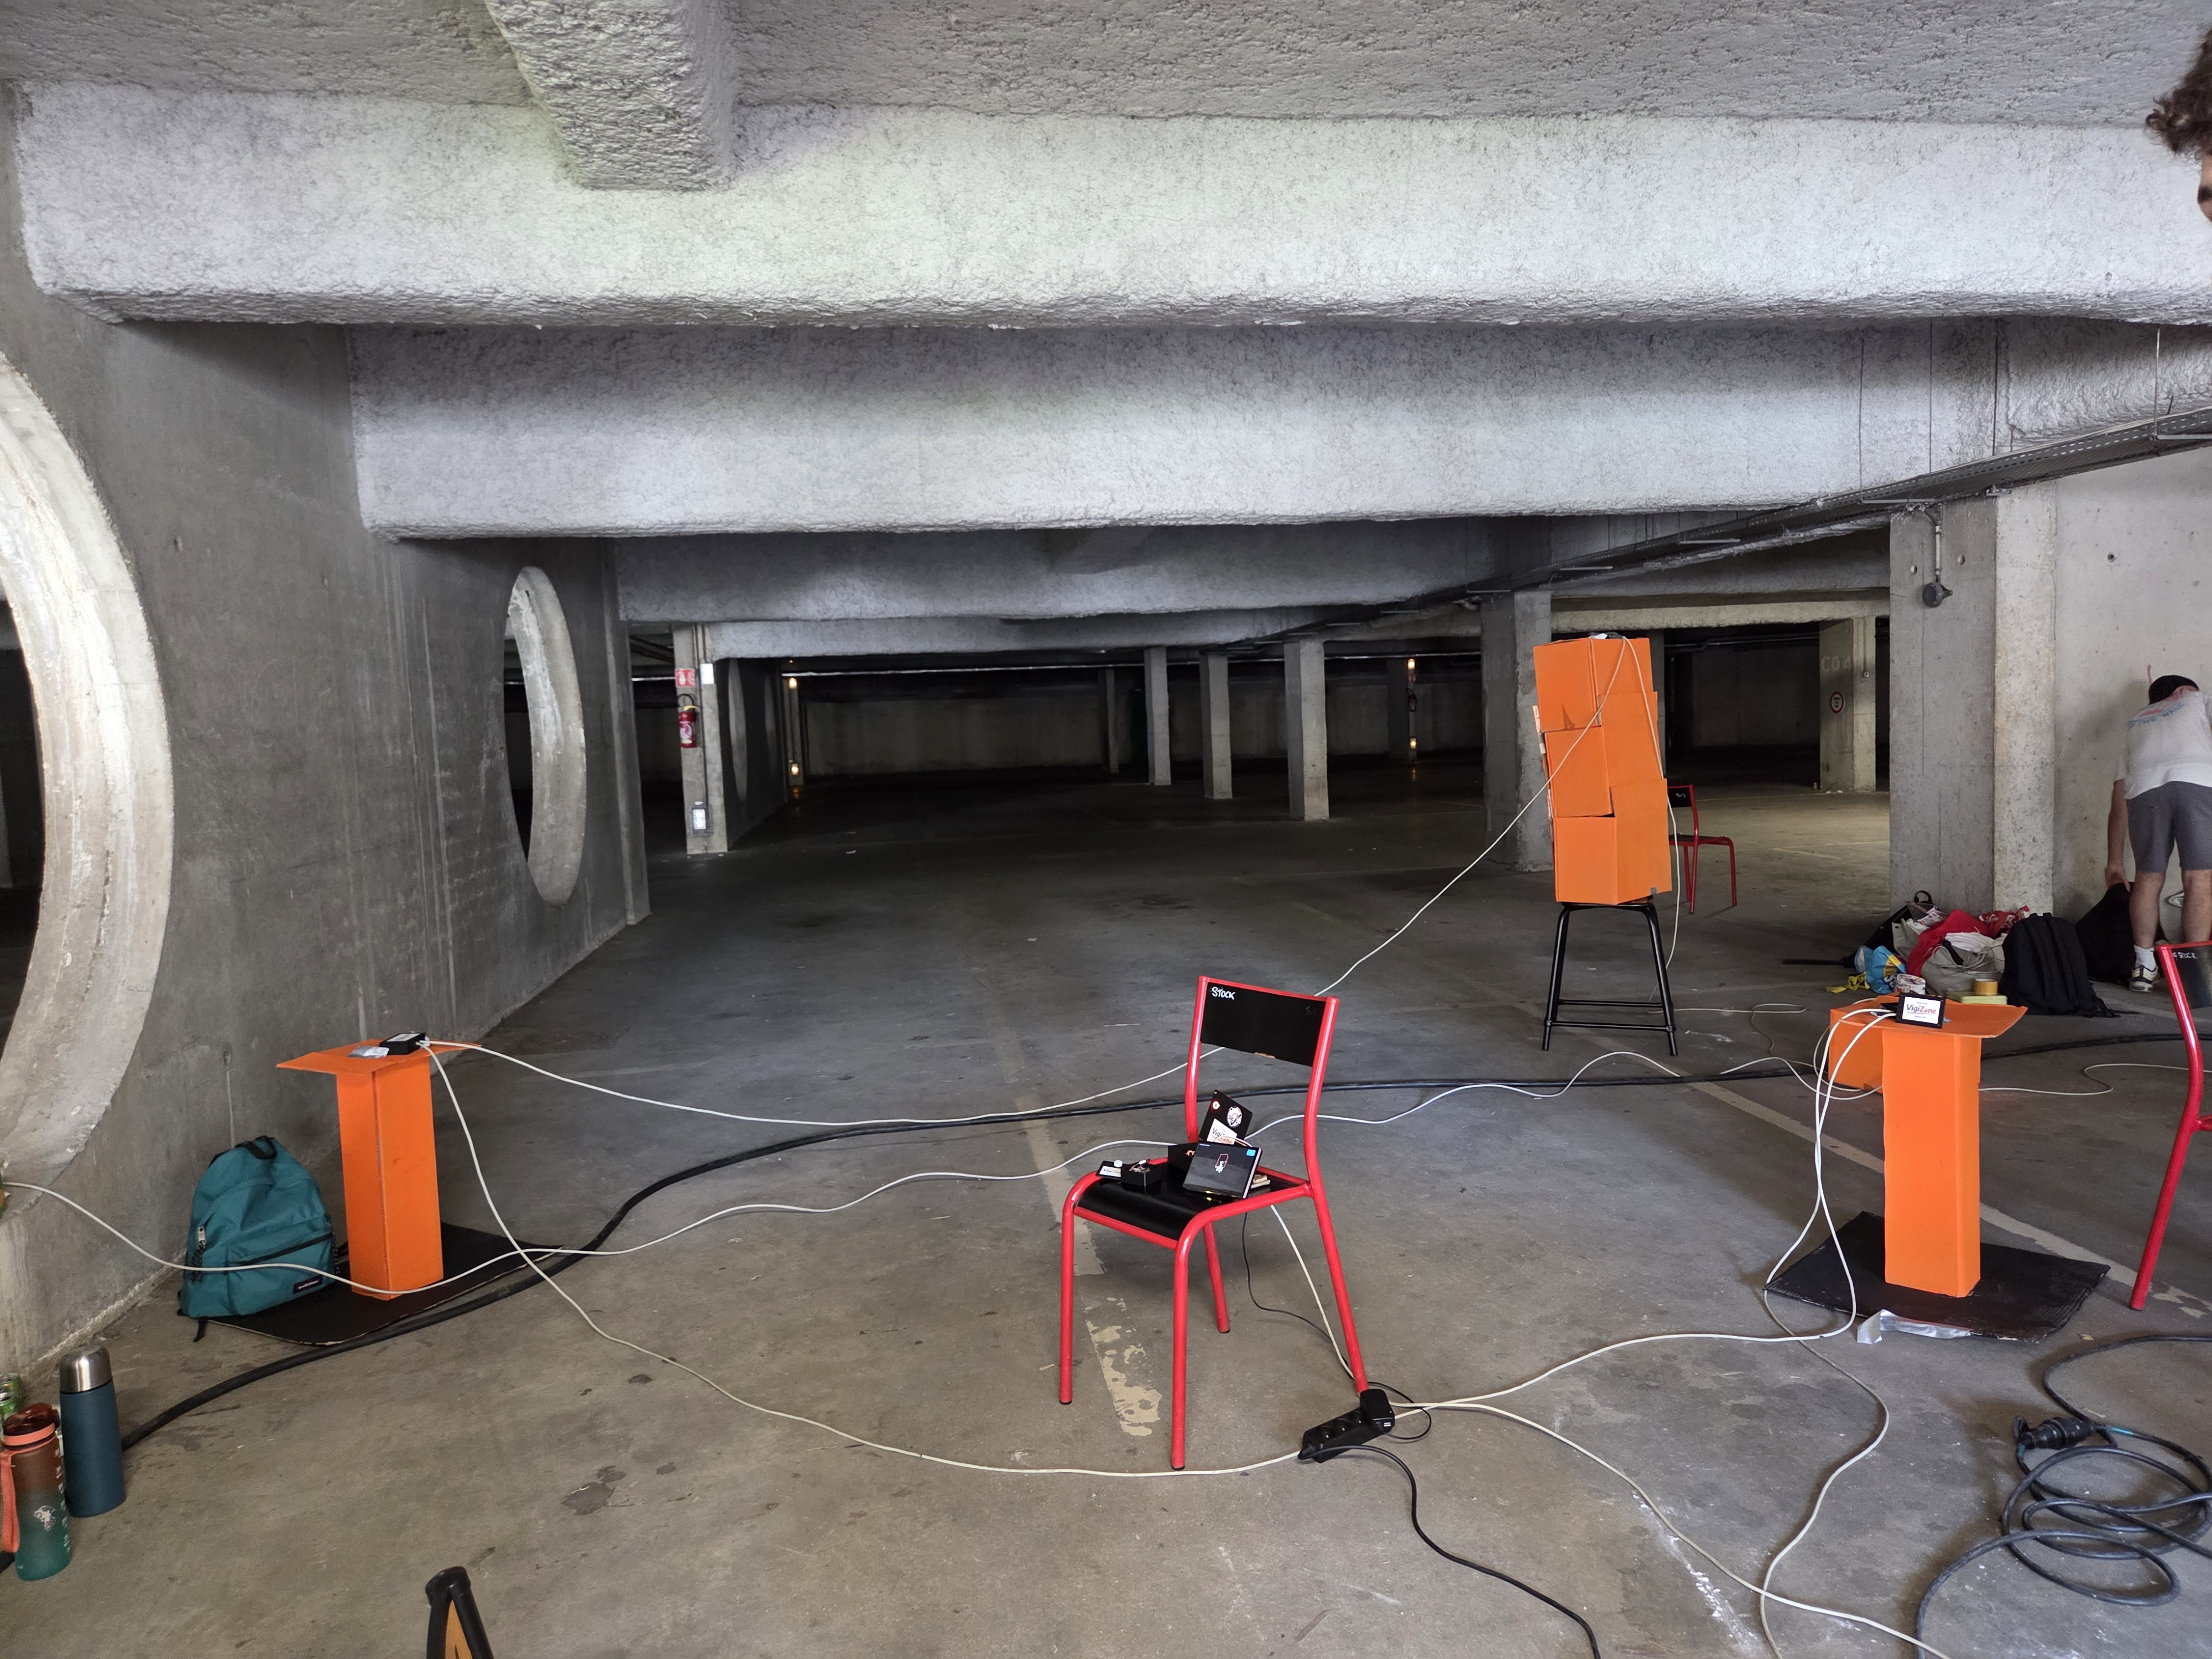
\includegraphics[width=0.65\columnwidth]{Figures/ImageSetupProto.jpg}
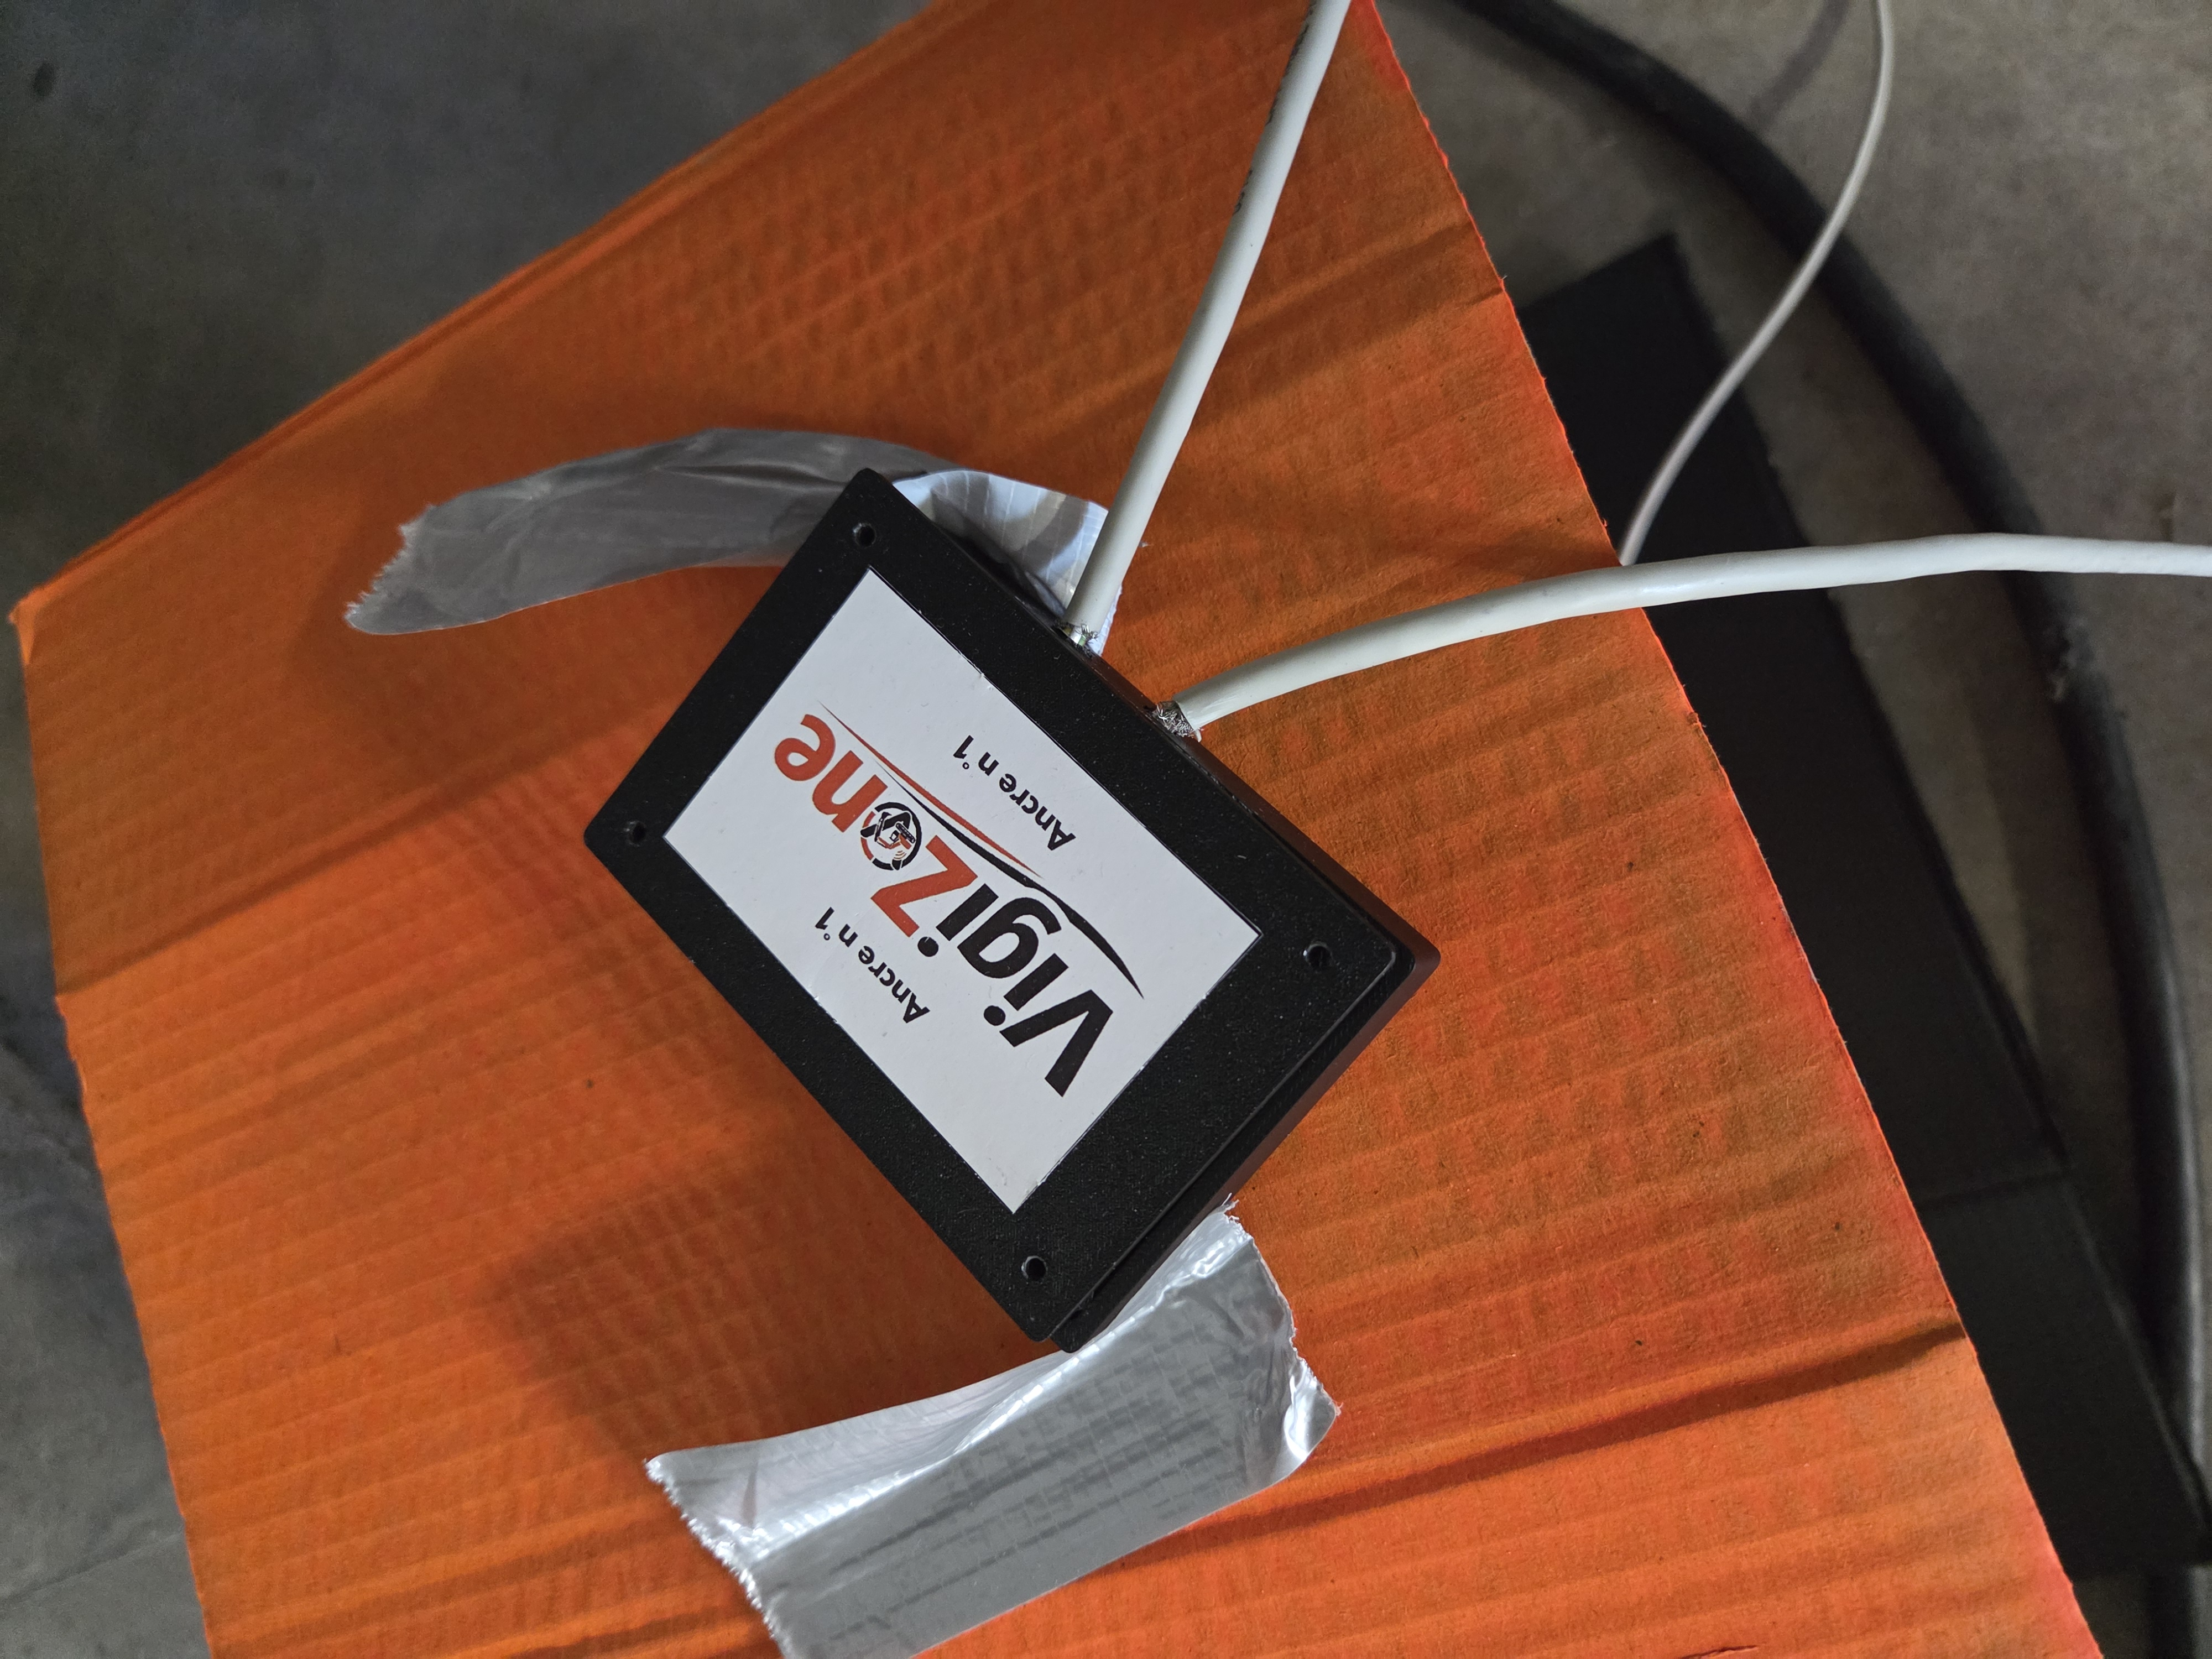
\includegraphics[width=0.65\columnwidth]{Figures/Ancre.jpg}
\caption[Installation du prototype en salle]{Dispositif de test en environnement contrôlé : simulation de l'engin par des supports cartonnés pour valider la géométrie en tétraèdre.}
\end{figure}

Les essais ont consisté à faire évoluer une personne muni d'un Tag autour de cette structure simulée, selon différentes trajectoires (approches frontales, déplacements latéraux, variations de vitesse) afin d'évaluer le comportement du système face à des cas d'usage standards.

\subsubsection{Analyse du suivi spatial}

Les données récoltées lors de ces simulations valident le fonctionnement nominal de la chaîne d'acquisition et de traitement :

\begin{itemize}
    \item \textbf{Précision de la détection UWB :} Dans ce milieu dépourvu de masses métalliques denses, l'algorithme des moindres carrés a calculé la position de l'opérateur avec une excellente précision. Le suivi des déplacements s'est avéré fluide et stable.
    \item \textbf{Traitement et affichage radar :} Les communications se sont bien déroulées. Le Tag a été retranscrit sur la vue de dessus avec des proportions exactes par rapport à la structure cartonnée simulée, démontrant l'indépendance de l'affichage par rapport aux variations d'altitude du capteur.
\end{itemize}

\begin{figure}[H]
\centering 

\includegraphics[width=0.7\columnwidth]{Figures/EcranFonctionnel.jpg}
\caption[Affichage radar en test]{Interface de l'écran affichant en temps réel le suivi de personnes}
\end{figure}

\subsubsection{Validation de la chaîne de sécurité}

L'évaluation de la fonctionnalité d'alerte critique a constitué la dernière phase du test. Une zone d'exclusion virtuelle a d'abord été créée autour de la structure simulée. L'opérateur a ensuite été invité à franchir volontairement cette frontière numérique avec son Tag. Le système a réagi sans latence perceptible, déclenchant simultanément l'alerte visuelle et sonore, et enregistrant l'événement dans le fichier d'historique sur la carte SD.

Si des tests ultérieurs sur un véritable engin (soumis aux réflexions de signaux dues à la carrosserie) demeurent nécessaires pour valider le produit fini, cette Preuve de Concept en salle confirme que le socle mathématique, la communication inter-microcontrôleurs et le logiciel d'interface répondent intégralement aux objectifs fixés.